 \documentclass[11pt,twoside,a4paper]{article}

\usepackage[polish]{babel}
\usepackage{polski}
\usepackage[utf8]{inputenc}
\usepackage[OT4]{fontenc}
\usepackage{tgtermes}	%Times New Roman
\usepackage[left=2.5cm,top=2.5cm,right=2.5cm,bottom=2.5cm,
headsep=0.5cm,headheight=1.0cm,marginpar=2cm,reversemp]{geometry}
\usepackage{fancyhdr}
\usepackage[table]{xcolor}  
\usepackage{graphicx}
\usepackage{amsmath}
\usepackage{amsthm,thmtools}
\usepackage[nottoc]{tocbibind}
\usepackage{ragged2e}
\usepackage{bbding}
\usepackage{makeidx}
\usepackage{titlesec}
%\usepackage{tcolorbox}
\usepackage{url} 
\usepackage{color}
\usepackage{setspace}
\usepackage[font=small,format=plain,labelfont=bf,up,textfont=it,up]{caption}
\usepackage{BeamerColor}
\usepackage{listings}
\usepackage{pdfpages}
\usepackage{hyperref}

\definecolor{mycolor1}{RGB}{0,0,128}
\definecolor{lightgray}{gray}{0.9}
\definecolor{lightlightgray}{gray}{0.95}
\definecolor{lightyellow}{RGB}{255,255,224}
\definecolor{lemonchiffon}{RGB}{255,250,205}



\newcommand{\mat}[1]{\boldsymbol{\mathrm{#1}}}

\hypersetup{
	pdftitle={Metody Programowania Robotów},
	pdfauthor={Pawe\l{} Malczyk, Pawe\l{} Tomulik},
	pdfkeywords={systemy operacyjne czasu rzeczywistego, QNX, robot},
	pdfsubject={Zestaw instrukcji laboratoryjnych QNX}
	pageanchor=true,
	breaklinks=true,
	plainpages=false,
	linktocpage=true
}
% zmiana nazw domyślnych 
\addto\captionspolish
{
	\renewcommand{\tablename}{Tabela}
	\renewcommand{\listtablename}{Spis tabel}
	\renewcommand{\bibname}{Piśmiennictwo}
	\renewcommand{\chaptername}{Laboratorium}
}


%\newtheoremstyle{mystyle}% name of the style to be used
%  {12pt}% measure of space to leave above the theorem. E.g.: 3pt
%  {12pt}% measure of space to leave below the theorem. E.g.: 3pt
%  {\itshape}% name of font to use in the body of the theorem
%  {6pt}% measure of space to indent
%  {\bfseries}% name of head font
%  {\newline}% punctuation between head and body
%  {.5em}% space after theorem head; " " = normal interword space
%  {}% Manually specify head
%\theoremstyle{mystyle}
%\newtheorem{example}{\color{black}Przykład}[section]


\declaretheoremstyle[
spaceabove=6pt, spacebelow=6pt,
headfont=\normalfont\bfseries,
notefont=\mdseries, 
notebraces={[}{]},
bodyfont=\itshape,
postheadspace=1em,
%qed=\qedsymbol
]{mystyle}
\declaretheorem[name=Przykład,numberwithin=subsection,style=mystyle]{example}
%\declaretheorem[name=Definition]{definition}



%\definecolor{lightyellow}{RGB}{255,255,224}
%\definecolor{lemonchiffon}{RGB}{255,250,205}

\lstset{ 
    language=C, % choose the language of the code
    alsolanguage=C++,
    basicstyle=\fontfamily{lmss}\selectfont\small\color{black},
    keywordstyle=\bfseries\color{blue}, % style for keywords
    numbers=left, % where to put the line-numbers
    numberstyle=\tiny, % the size of the fonts that are used for the line-numbers     
    backgroundcolor=\color{lemonchiffon},
%    backgroundcolor=\color{lightgray},
    showspaces=false, % show spaces adding particular underscores
    showstringspaces=false, % underline spaces within strings
    showtabs=false, % show tabs within strings adding particular underscores
    frame=single, % adds a frame around the code
    tabsize=2, % sets default tabsize to 2 spaces
    rulesepcolor=\color{gray},
    rulecolor=\color{black},
    captionpos=t, % sets the caption-position to bottom
    breaklines=true, % sets automatic line breaking
    breakatwhitespace=false, 
    xleftmargin=20pt,
    xrightmargin=20pt,
    aboveskip=12pt,
    belowskip=12pt,
%   frameround=tttt,
}
\renewcommand*\lstlistingname{Kod źródłowy}
\renewcommand{\qedsymbol}{\rule{1ex}{1ex}}
\lstset{framexleftmargin=5mm, frame=shadowbox, rulesepcolor=\color{lightgray}}
\lstset{
extendedchars=\true,
inputencoding=utf8
}

%\lstset{language=Fortran, numbers=left, numberstyle=\tiny, stepnumber=1, numbersep=0pt, tabsize=5,keywordstyle=\color{black}\bfseries,aboveskip=10pt,belowskip=36pt,
%xleftmargin=20pt,xrightmargin=20pt}
%\lstset{emph={Procedura,Oblicz},emphstyle={\color{black}\bfseries},
%label=list1}
%\renewcommand*\lstlistingname{Tekst programu}
%
%\begin{lstlisting}[frame=lines,caption={Pseudokod algorytmu dziel i~zdobywaj z~dyrektywami kompilatora OpenMP}]
%\end{lstlisting}


\renewcommand{\labelitemi}{$\bullet$}
%\renewcommand{\labelitemii}{$\cdot$}
%\renewcommand{\labelitemiii}{$\diamond$}
%\renewcommand{\labelitemiv}{$\ast$}

% Wielkosc wciecia akapitowego
\parindent=0.5cm
% Odstepy miedzy akapitami
\parskip=6pt

% Uklad strony
% \pagestyle{empty}
\fancyhead{}
\pagestyle{fancy}
% Naglowki na stronie parzystej (E) i nieparzystej (O) , Right Left Center
%\fancyhead[CO]{\small \nouppercase{\textbf\rightmark}}
%\fancyhead[CE]{\small \nouppercase{\textbf\leftmark}}

%\lhead{\textbf{\small{\leftmark}}}
%\rhead{\small{Pawel Malczyk}}
%\lfoot{\textbf{\tiny{Konspekt do Podstaw Automatyki i Sterowania II}}}
%\rfoot{}

\fancyhead[CE]{\small \nouppercase{\textbf\leftmark}}
\fancyhead[CO]{\small \nouppercase{\textbf{Metody Programowania Robotów (QNX RTOS)}}}

\fancyfoot[RE,RO]{\footnotesize Paweł Malczyk, Paweł Tomulik}
\fancyfoot[LE,LO]{\footnotesize Rozpowszechnianie bez zgody autorów zabronione}
%\fancyfoot[RE,RO]{\footnotesize Rozpowszechnianie bez zgody autorów zabronione}

\linespread{1.0}
\title{\vspace{4.25cm}\Huge{\textbf{Metody Programowania Robotów}} \\ \vskip10pt\LARGE{\textit{Zestaw instrukcji laboratoryjnych do programowania aplikacji w~systemie operacyjnym czasu rzeczywistego QNX}}} 
\author{\Large{\textbf{Paweł Malczyk, Paweł Tomulik}}\vspace{0.5cm} \\ Zakład Teorii Maszyn i Robotów \\
Instytut Techniki Lotniczej i Mechaniki Stosowanej \\
Wydział Mechaniczny Energetyki i Lotnictwa \\
Politechnika Warszawska \\
{\href{mailto:pmalczyk@meil.pw.edu.pl}{pmalczyk@meil.pw.edu.pl}}, \href{mailto:ptomulik@meil.pw.edu.pl}{ptomulik@meil.pw.edu.pl} \\ www: \href{http://ztmir.meil.pw.edu.pl}{http://ztmir.meil.pw.edu.pl}}
\date{października 2015 r.}

\linespread{1.3}

%  \titleformat{<command>}[<shape>]{<format>}{<label>}{<sep>}{<before-code>}[<after-code>]


\titleformat
{\section}
[display]
{\color{black}\normalfont\Large\bfseries\centering}
{\color{black}{\rule{\textwidth}{1pt}\\ \LARGE Laboratorium~\thesection}}
{-1em}
{
    %\rule{\textwidth}{1pt}
    \vspace{1ex}
    \centering
}
[
\vspace{-2.5ex}%
\rule{\textwidth}{0.3pt}
] % after-code

\titleformat{\subsection}
{\color{black}\normalfont\Large\bfseries}
{\color{black}\thesubsection}{1em}{}

\newenvironment{myitemize}
{ \begin{itemize}
    \setlength{\itemsep}{0pt}
    \setlength{\parskip}{0pt}
    \setlength{\parsep}{0pt}     }
{ \end{itemize}                  } 

\newenvironment{myenumerate}
{ \begin{enumerate}
    \setlength{\itemsep}{0pt}
    \setlength{\parskip}{0pt}
    \setlength{\parsep}{0pt}     }
{ \end{enumerate}                  } 


\begin{document}
\maketitle
\cleardoublepage 

\section{Podstawy obsługi systemu operacyjnego QNX RTOS}

\subsection{Powłoka}

Powłoka: 

\begin{myitemize}
\item Interpreter poleceń użytkownika
\item Pośredniczy między użytkownikiem a systemem
\item Środowisko pracy użytkownika w systemie
\item Przetwarza pojedyncze polecenie lub skrypty
\end{myitemize}


\begin{example}[Przykład prostej komendy] \label{ex:prostakomenda} 

Polecenia można wydawać powłoce z wiersza poleceń (terminala, konsoli) wpisując ich nazwy.

\begin{lstlisting}[language=bash]
# ls
\end{lstlisting}

Komenda wyświetla zawartość bieżącego katalogu.  
\end{example}

\begin{example}[Przykład komendy z~argumentami]\label{ex:prostakomenda2} 
%\addcontentsline{toc}{subsubsection}{Przykład \ref{ex:prostakomenda2}}

Komenda wyświetla zawartość bieżącego katalogu wraz ze szczegółowymi informacjami nt. obiektów. Argumenty (\lstinline{-l}) zmieniają zachowanie komendy prostej.

\begin{lstlisting}[language=bash]
# ls -l 
\end{lstlisting}


Formalna składnia komendy z argumentami:

\begin{lstlisting}[language=bash]
# command argument1 argument2 argument3 ... argumentN
\end{lstlisting}
\end{example}

\begin{example}[Przykład złożonej komendy]\label{ex:prostakomenda3} 

Komendy proste i~komendy proste z~argumentami możemy łączyć. Separatorem poleceń jest średnik (\lstinline{;}). 


\begin{lstlisting}[language=bash]
# date ; ls
\end{lstlisting}

Formalna składnia złożonej komendy: 

\begin{lstlisting}[language=bash]
# command1; command2; command3; ... argumentN
\end{lstlisting}
\end{example}

\begin{example}[Logowanie do systemu z wiersza poleceń]\label{ex:prostakomenda4} 


Aby zalogować się do systemu z wiersza poleceń używamy polecenia \lstinline{login}.

\begin{lstlisting}[language=bash]
# login
# login: root
\end{lstlisting}

Polecenie uzyskuje od użytkownika jego nazwę oraz hasło, które następnie weryfikuje z danymi zawartymi w pliku \lstinline{/etc/passwd}, który możemy podejrzeć poleceniem \lstinline{cat}. 
\end{example}


\begin{example}[Plik definiujący użytkowników systemu]\label{ex:prostakomenda5} 


Po zalogowaniu przez polecenie \lstinline{login} wywoływana jest powłoka (\lstinline{/bin/sh}). Następnie w fazie inicjalizacji, ustawiane są parametry pracy powłoki. Na ogół jest to proces dwuetapowy, w~którym interpretowane są pliki \lstinline{/etc/profile} oraz \lstinline{.profile} z domowego katalogu. 

\begin{lstlisting}[language=bash]
# cat /etc/passwd
\end{lstlisting}
\end{example}

\begin{example}[Wejście i wyjście z powłoki]\label{ex:prostakomenda6} 


Powłoka wykonuje polecenia użytkownika. Kiedy powłoka wyświetla znak zachęty, który w domyślnym shell-u (Bourne shell) w systemie QNX jest znak \lstinline{#} dla użytkownika \lstinline{root}, to czeka na polecenia użytkownika. Możemy uruchomić powłokę w takim trybie. Sytuację tę ilustruje poniższy przykład.  


\begin{lstlisting}[language=bash]
# /bin/sh
#
# exit
\end{lstlisting}

Aby wyjść z powłoki należy użyć polecenia \lstinline{# exit}. 
\end{example}

\begin{example}[Obsługa edytora tekstu vi]\label{ex:vi} 


Edytor \lstinline{vi} jest edytorem tekstowym często występującym w~systemach Unix. Aby uruchomić edytor należy wpisać komendę: 

\begin{lstlisting}[language=bash]
# vi
\end{lstlisting}

 Edytor \lstinline{vi} jest edytorem modalnym. Oznacza to, że może znajdować się w~dwóch stanach: \textbf{trybie edycji} lub \textbf{trybie poleceń}. 
 
\begin{itemize}
\item Przejście do trybu edycji poprzez wydanie polecenia \lstinline{i} (insert) lub \lstinline{a} (append).
\item Przejcie z~trybu edycji do trybu poleceń odbywa się poprzez naciśnięcie klawicza \lstinline{Esc}. 
\end{itemize}

Polecenia edytora \lstinline{vi} składają się z~kilku grup. Przedstawiono je zbiorczo w~postaci krótkiej instrukcji na stronie~\pageref{viRef}.
\end{example} 

\clearpage  
\phantomsection
{\label{viRef}
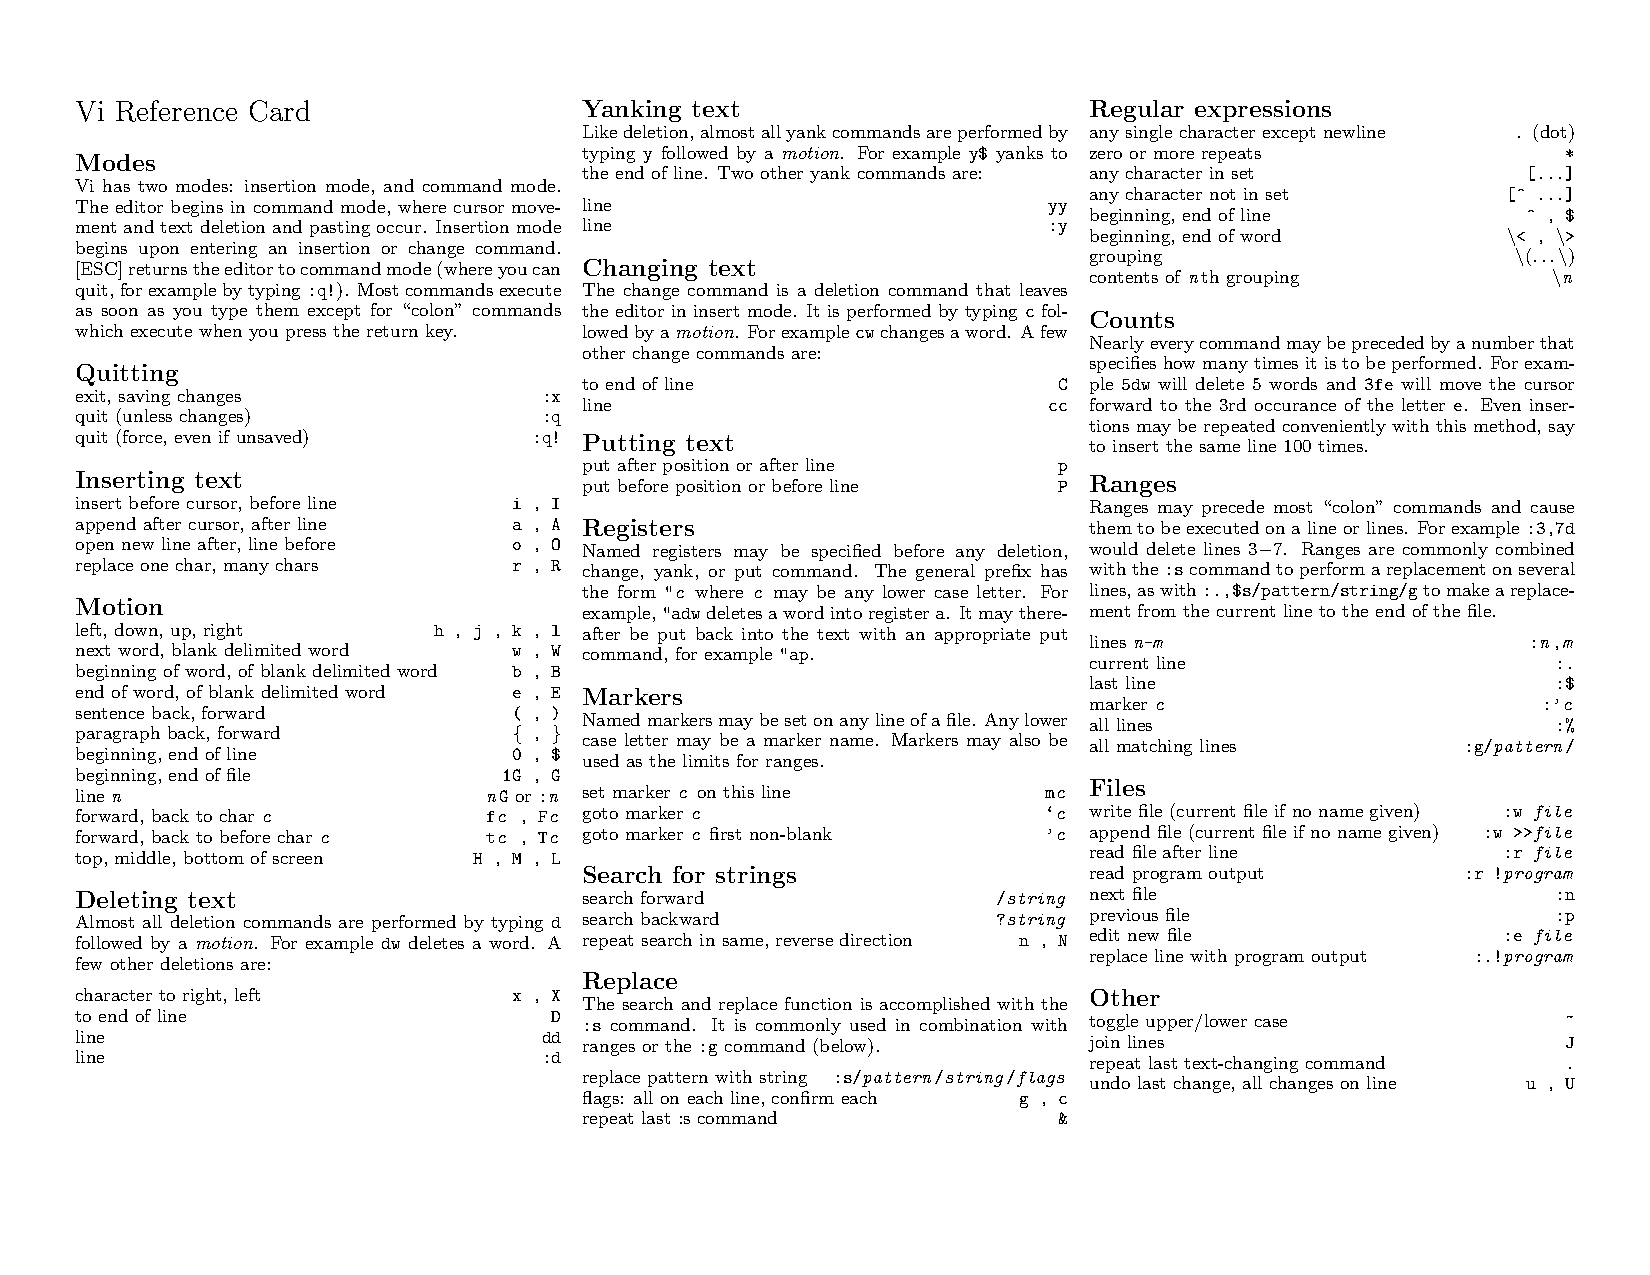
\includepdf[scale=0.95,pages={1},pagecommand={\thispagestyle{fancy}},pagecommand={\thispagestyle{fancy}{\label{subsec:vi}}},lastpage=1,angle=90]{img/viRef.pdf}
}



\begin{example}[Utworzenie i~uruchomienie skryptu] \label{ex:prostakomenda7} 


Powłoka, jako interpreter, wykonuje pewien program.  Kolejne komendy programu mogą być wpisywane na bieżąco w~terminalu lub cały program może być dostarczony do powłoki w~postaci skryptu. Należy utworzyć plik o~nazwie \lstinline{skrypt} edytorem tekstu \lstinline{vi} o~treści:

\begin{lstlisting}[language=bash]
date ; ls
\end{lstlisting}

W~następnej kolejności uruchomić skrypt powłoki wydając polecenie: 

\begin{lstlisting}[language=bash]
# /bin/sh skrypt
\end{lstlisting}

Przykład ilustruje skrypt powłoki. Na ogół skrypty składają się z plików, w których są zapisane komendy, interpretowane przez powłokę. Skrypt można uruchomić wpisując w wiersz poleceń jego nazwę. Jednak bezpośrednie wpisanie jego nazwy kończy się niepowodzeniem:

\begin{lstlisting}[language=bash]
# ./skrypt
sh: ./skrypt: cannot execute - Permission denied
\end{lstlisting}

W tej sytuacji należy zapewnić, aby skrypt miał odpowiednie atrybuty oraz upewnić się, że uruchamiany jest właściwy interpreter poleceń. Aby zmienić atrybuty pliku należy użyć następującego polecenia:

\begin{lstlisting}[language=bash]
# chmod a+x ./skrypt
\end{lstlisting}

Uruchomić \lstinline{skrypt} w~linii poleceń. 
\end{example}


\begin{example}[Prosty skrypt powłoki]\label{ex:prostakomenda8} 


Należy także uzupełnić plik \lstinline{skrypt}, tak, żeby miał postać:

\begin{lstlisting}[language=bash]
#!/bin/sh
# wypisz date i wyswietl zawartosc katalogu
date ; ls
\end{lstlisting}

Znak \lstinline{#} stanowi znak komentarza w~skrypcie. Wiersze zaczynające się od tego znaku są ignorowane przez interpreter poleceń i~traktowane jako komentarz, oprócz pierwszej linii z~komendą \lstinline{#!/bin/sh}. Pierwsza linia kodu przekazuje informacje o~rodzaju powłoki, która powinna wykonać skrypt. 
\end{example}


\begin{example}[Prosty skrypt powłoki]\label{ex:prostakomenda9} 

Dokumentacja systemu jest dostępna w formie elektronicznej na stronach \href{www.qnx.com}{www.qnx.com}. Skrócony opis interesującego nas polecenia systemowego uzyskujemy poprzez wpisanie w okno terminala polecenia \lstinline{use polecenie}, np.:

\begin{lstlisting}[language=bash]
# use date
\end{lstlisting}
\end{example}

\subsection{System plików} 

W systemie QNX Neutrino prawie wszystkie zasoby są plikami. Dane, urządzenia, bloki pamięci, a nawet pewne usługi są reprezentowane przez abstrakcję plików. Mechanizm plików pozwala na jednolity dostęp do zasobów zarówno lokalnych, jak i~zdalnych, za pomocą poleceń i programów usługowych wydawanych z okienka poleceń. Typowe drzewo plików w~systemie QNX przedstawiono na rysunku~\ref{fig:drzewo}. 

\begin{figure}[!h]
\centering
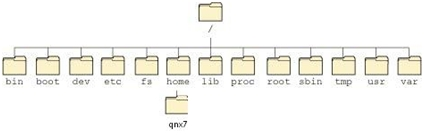
\includegraphics[width=0.75\textwidth]{img/systemplikow}
\caption{Drzewo plików w systemie QNX}
\label{fig:drzewo}
\end{figure}

\begin{myitemize}
\item Katalog główny \lstinline{/} jest miejscem montowania twardego dysku lub pamięci flash.  
\item \lstinline{/bin} - zawiera podstawowe komendy systemowe (np. \lstinline{ls}, \lstinline{chmod}). 
\item \lstinline{/boot} - zawiera pliki i katalogi związane z obrazami systemu operacyjnego.
\item \lstinline{/dev} - katalog przynależy do menadżera zasobów, w którym przechowywane są informacje o urządzeniach dostępnych w systemie. 
\item \lstinline{/etc} - zawiera pliki i programy używane do administracji i konfiguracji systemu.
\item \lstinline{/fs} - w katalogu są montowane dodatkowe systemy plików.
\item \lstinline{/home} - katalogi domowe użytkowników.
\item \lstinline{/lib} - zawiera współdzielone biblioteki używane przez inne programy, procesy. 
\item \lstinline{/proc} - katalog, w którym są zawarte informacje o procesach i przestrzeni nazw. 
\item \lstinline{/root} - katalog domowy dla użytkownika root.
\item \lstinline{/sbin} - zawiera niezbędne pliki wykonywalne (np. sterowniki, programy inicjujące, konfiguracyjne, menadżery).
\item \lstinline{/tmp} - zawiera pliki tymczasowe.
\item \lstinline{/usr} - zawiera współdzielone dane, tylko do odczytu.
\item \lstinline{/var} - zawiera zmienne dane (np. cache, logi). 
\end{myitemize}

W systemie QNX występują różne typy plików. Ich zestawienie przedstawiono w~tabeli \ref{tab:typyplikow}. 


\begin{table}[h!]
\centering
\caption{Typy plików w~systemie QNX}
\setlength{\arrayrulewidth}{1pt}
\setlength{\tabcolsep}{6pt}
\renewcommand{\arraystretch}{1.2}
\begin{tabular}{ |p{0.15\textwidth}|p{0.3\textwidth}|p{0.4\textwidth}| }
\hline \rowcolor{gray}
\textbf{Oznaczenie} & \textbf{Typ pliku} & \textbf{Opis} \\ \hline
\mbox{\lstinline{d}} & Katalog (ang. directory) & Plik zawierający inne pliki i katalogi. \\ \hline
\mbox{\lstinline{l}} & Dowiązanie symboliczne (ang. symbolic link) & Dodatkowa nazwa pliku, który jest umieszczony w innym miejscu. \\ \hline
\mbox{\lstinline{n}} & Plik specjalny & Np. blok pamięci współdzielonej. \\ \hline
\mbox{\lstinline{c}} & Specjalny plik znakowy (ang. charakter device) & Urządzenie z dostępem znakowym (konsola, porty szeregowe, równoległe). \\ \hline
\mbox{\lstinline{p}} & Plik specjalny FIFO & Bufor cykliczny w pamięci operacyjnej. \\ \hline
\mbox{\lstinline{b}} & Specjalny plik blokowy (ang. block device) & Urządzenie z dostępem blokowym (dysk, partycja dyskowa). \\ \hline
\mbox{\lstinline{s}} & Gniazdko (ang. socket)	 & Plik komunikacji sieciowej. \\ \hline
\end{tabular}
\label{tab:typyplikow}
\end{table}


Pliki są zorganizowane w katalogi. Katalogi mają strukturę drzewa z korzeniem \lstinline{/} (\lstinline{root}). Aby wskazać na konkretny obiekt w systemie plików, należy podać jego ścieżkę. Rozróżniamy ścieżki absolutne i~względne. Ścieżka absolutna zaczyna się od znaku \lstinline{/} , np. \lstinline{/etc/passwd}. Ścieżka relatywna zaczyna się od znaku innego niż \lstinline{/} , np. \lstinline{etc/passwd} .


\begin{example}[Wylistowanie zawartości katalogu]\label{ex:wylistowanie} 

Pokazać zawartość bieżącego katalogu: 

\begin{lstlisting}[language=bash]
# ls -l 
total 419571
drwxr-xr-x   2 root      root           3072 Feb 23  2014 bin
drwxr-xr-x   4 root      root           1024 Feb 23  2014 boot
dr-xr-xr-x   2 root      root              0 Oct 22 15:07 dev
drwxr-xr-x  10 root      root           3072 Feb 23  2014 etc
drwxr-xr-x   2 root      root           1024 Feb 23  2014 home
drwxr-xr-x   4 root      root           5120 Feb 23  2014 lib
drwxr-xr-x   3 root      root           1024 Feb 23  2014 libexec
dr-xr-xr-x   2 root      root      214798336 Oct 22 15:07 proc
drwxr-xr-x   2 root      root           1024 Sep 30 21:43 root
drwxr-xr-x   2 root      root           3072 Feb 23  2014 sbin
-rw-rw-rw-   1 root      root             11 Oct 22 12:14 skrypt
drwxr-xr-x   2 root      root           1024 Oct 22 12:30 tmp
drwxr-xr-x   7 root      root           1024 Feb 23  2014 usr
drwxr-xr-x   4 root      root           1024 Feb 23  2014 var
\end{lstlisting}

Pokazać zawartość innego katalogu: 

\begin{lstlisting}[language=bash]
# ls -la /usr/
\end{lstlisting}

Argument \lstinline{-l} służy do listowania w formacie tzw. długim, natomiast argument \lstinline{-a} do listowania ukrytych plików. Sprawdzić inne parametry polecenia ls następująco:  

\begin{lstlisting}[language=bash]
# use ls
\end{lstlisting}
\end{example}

\begin{example}[Obejrzenie zawartości pliku]\label{ex:obejrzenie} 

Oprócz listowania zawartości katalogów, istotna jest możliwość oglądania zawartości plików (np. skryptowych):

\begin{lstlisting}[language=bash]
# cat /skrypt
# cat -n /skrypt			# -n numerowanie linii
# cat -n /etc/passwd
\end{lstlisting}
\end{example}


\begin{example}[Wyświetlanie liczby wierszy, słów i~bajtów zawartych w pliku]\label{ex:wys} 

Aby uzyskać informację o całkowitej liczbie linii, słów i~znaków, zawartych w pliku można użyć polecenie \lstinline{wc} (ang. word count): 

\begin{lstlisting}[language=bash]
# wc /skrypt
\end{lstlisting}

Dostępne argumenty polecenia przedstawiono w~tabeli \ref{tab:opcjeWC}. 


\begin{table}[h!]
\centering
\caption{Opcje polecenia wc}
\setlength{\arrayrulewidth}{1pt}
\setlength{\tabcolsep}{6pt}
\renewcommand{\arraystretch}{1.2}
\begin{tabular}{ |p{0.15\textwidth}|p{0.4\textwidth}|}
\hline \rowcolor{gray}
\textbf{Argumenty} & \textbf{Opis} \\ \hline
\mbox{\lstinline{-l}} & Oblicza liczbę linii \\ \hline
\mbox{\lstinline{-w}} & Oblicza liczbę słów \\ \hline 
\mbox{\lstinline{-m}} & Oblicza liczbę znaków \\ \hline
\mbox{\lstinline{-c}} & Oblicza liczbę znaków  \\ \hline
\end{tabular}
\label{tab:opcjeWC}
\end{table}

\begin{example}[Poruszanie się po systemie plików]

System operacyjny jest wyposażony w zestaw instrukcji, które umożliwiają poruszanie się po drzewie plików. Najważniejsze zestawiono w tabeli~\ref{tab:poruszanie} i~zilustrowano w przykładzie.

\begin{table}[h!]
\centering
\caption{Poruszanie się po systemie plików}
\setlength{\arrayrulewidth}{1pt}
\setlength{\tabcolsep}{6pt}
\renewcommand{\arraystretch}{1.2}
\begin{tabular}{ |p{0.15\textwidth}|p{0.4\textwidth}|}
\hline \rowcolor{gray}
\textbf{Polecenie} & \textbf{Opis} \\ \hline
\mbox{\lstinline{pwd}} & Wyświetlenie nazwy katalogu bieżącego (ang. print working directory) \\ \hline 
\mbox{\lstinline{cd}}  & Zmiana katalogu bieżącego (ang. change directory) \\ \hline
\mbox{\lstinline{cd..}} & Przejście do katalogu nadrzędnego \\ \hline 
\mbox{\lstinline{cd /}} & Przejście do katalogu głównego \\ \hline 
%\mbox{\lstinline{cd ~}} &	Przejście do katalogu domowego \\ \hline 
\end{tabular}
\label{tab:poruszanie}
\end{table}
\end{example}



Wprowadzić następujące komendy w~wierszu poleceń. 

\begin{lstlisting}[language=bash]
# pwd			# Nazwa katalogu biezacego 
/ 
# cd /usr			# Przejscie do katalogu uzytkownika
# pwd 
/usr 
# cd ..			# Przejscie do katalogu nadrzednego 
# pwd
/
# ls .			# Wylistowanie nazw plikow w biezacym katalogu 
...
# ls -l 			# Wylistowanie ze szczegolami
\end{lstlisting}
\end{example}

\begin{example}[Utworzenie i kasowanie katalogów]

Pliki w systemie plików można tworzyć i usuwać. Katalogi można również modyfikować. Najczęściej używane polecenia służą do tworzenia, kopiowania, przenoszenia oraz usuwania katalogów. Zestawienie podstawowych poleceń podano w tabeli~\ref{tab:tworziusun}.

\begin{table}[h!]
\centering
\caption{Tworzenie i usuwanie katalogów i~plików}
\setlength{\arrayrulewidth}{1pt}
\setlength{\tabcolsep}{6pt}
\renewcommand{\arraystretch}{1.2}
\begin{tabular}{ |p{0.15\textwidth}|p{0.4\textwidth}|}
\hline \rowcolor{gray}
\textbf{Polecenie} & \textbf{Opis} \\ \hline
\mbox{\lstinline{touch plik}} & Utworzenie pustego pliku lub zmiana daty modyfikacji istniejącego \\ \hline 
\mbox{\lstinline{cd}}  & Zmiana katalogu bieżącego (ang. change directory) \\ \hline
\mbox{\lstinline{rm [-Rfi] plik}} & Usunięcie pliku: \mbox{\lstinline{-i}} - żądanie potwierdzenie; \mbox{\lstinline{-f}} - bezwarunkowe kasowanie pliku; \mbox{\lstinline{-R}} - kasowanie zawartości katalogu z~podkatalogami  \\ \hline 
\mbox{\lstinline{mkdir katalog}} & Utworzenie katalogu o nazwie \mbox{\lstinline{katalog}} \\ \hline 
\mbox{\lstinline{rmdir katalog}} &	Usunięcie katalogu o nazwie \mbox{\lstinline{katalog}}  \\ \hline 
\end{tabular}
\label{tab:tworziusun}
\end{table}

Sprawdzić działanie następujących komend: 

\begin{lstlisting}[language=bash]
# pwd			# Nazwa katalogu biezacego 
/
# cd /home			# Przejdz do katalogu home
# mkdir katalog			# Utworzenie katalogu
# cd katalog			# Przejdz do katalogu
# mkdir podkatalog			# Utworzenie podkatalogu
# touch plik			# Utworzenie pustego pliku
# touch plik2			# Utworzenie pustego pliku
# rm plik2			# Usuniecie pustego pliku
# rmdir podkatalog			# Usuniecie podkatalogu
# cd .. 			# Wyjscie do katalogu nadrzednego 
# rmdir katalog 			# Proba usuniecia podkatalogu
katalog/: Directory not empty 
# rm -Ri katalog			# Usuniecie rekursywne z potwierdzeniem
rm: remove katalog/plik? (y/N) y
rm: remove directory katalog? (y/N) y
\end{lstlisting}

\end{example}


\begin{example}[Przenoszenie i~kopiowanie katalogów i~plików]

Pliki i~katalogi można kopiować i~przenosić. Zestawienie najważniejszych komend przedstawiono w~tabeli~\ref{tab:przenos}. 

\begin{table}[h!]
\centering
\caption{Przenoszenie i~kopiowanie katalogów i~plików}
\setlength{\arrayrulewidth}{1pt}
\setlength{\tabcolsep}{6pt}
\renewcommand{\arraystretch}{1.2}
\begin{tabular}{ |p{0.2\textwidth}|p{0.4\textwidth}|}
\hline \rowcolor{gray}
\textbf{Polecenie} & \textbf{Opis} \\ \hline
\mbox{\lstinline[deletekeywords={if}]{mv [-if] zrodlo cel}} & Przenoszenie lub zmiana nazwy plików: \mbox{\lstinline{-i}} - żądanie potwierdzenia, gdy plik docelowy może być nadpisany; \mbox{\lstinline{-f}} - bezwarunkowe skopiowanie pliku \\ \hline 
\mbox{\lstinline{cp [-ifR] zrodlo cel}}  & Kopiowanie plików: \mbox{\lstinline{-i}} - żądanie potwierdzenia, gdy plik docelowy może być nadpisany; \mbox{\lstinline{-f}} - bezwarunkowe skopiowanie pliku; \mbox{\lstinline{-R}} - kopiowanie zawartości katalogu z podkatalogami \\ \hline
\end{tabular}
\label{tab:przenos}
\end{table}

Sprawdzić działanie następujących komend: 

\begin{lstlisting}[language=bash]
# pwd
/home 
# mkdir katalog
# cd katalog 
# touch pliczek
# cd ..
# mv ./katalog/pliczek .			# Przeniesienie do katalogu biezacego
# mv pliczek plik.dat			# Zmiana nazwy pliku
# cp plik.dat katalog			# Skopiowanie pliku do katalogu
# cp -Ri katalog katalog2			# Skopiowanie katalogu do katalogu2 razem z zawartoscia
\end{lstlisting}
\end{example}


\begin{example}[Zmiana atrybutów pliku]

Pliki w systemie mają określonych właścicieli, grupy użytkowników, a także zestawy atrybutów do nich przypisanych. System umożliwia dostęp do plików w trybie odczytu, zapisu lub wykonania. Symboliczne oznaczenia praw dostępu do pliku są następujące:

\begin{myitemize}
\item \lstinline{r} - prawo odczytu (ang. read)
\item \lstinline{w} - prawo zapisu (ang. write)
\item \lstinline{x} - prawo wykonania (ang. execute)
\end{myitemize}

Prawa te mogą być zdefiniowane dla właściciela pliku, grupy, do której on należy i wszystkich innych użytkowników.

\begin{myitemize}
\item \lstinline{u} - właściciel pliku (ang. user)
\item \lstinline{g} - grupa (ang. group)
\item \lstinline{o} - inni użytkownicy (ang. other)
\end{myitemize}

Aby obejrzeć właściciela pliku oraz atrybuty wykonajmy następujące polecenie:

\begin{lstlisting}[language=bash]
# ls -l /home/plik.dat
-rw-rw-rw- 1 root root 0 Oct 22 11:41 /home/plik.dat
\end{lstlisting}

W~terminalu wyświetlone zostały w~kolejności atrybuty dla właściciela (\lstinline{rw-}), grupy (\lstinline{rw-}) oraz innych użytkowników (\lstinline{rw-}); wskazano także liczbę dowiązań \lstinline{1}, nazwę właściciela pliku \lstinline{root}, nazwę grupy \lstinline{root}, rozmiar pliku \lstinline{0}, datę utworzenia \lstinline{Oct 22 11:41} oraz nazwę pliku \lstinline{home/plik.dat}. 


Atrybuty plików oraz ich właścicieli można zmieniać - zobacz tabela \ref{tab:zmien}. 

\begin{table}[h!]
\centering
\caption{Tworzenie i usuwanie katalogów i~plików}
\setlength{\arrayrulewidth}{1pt}
\setlength{\tabcolsep}{6pt}
\renewcommand{\arraystretch}{1.2}
\begin{tabular}{ |p{0.15\textwidth}|p{0.4\textwidth}|}
\hline \rowcolor{gray}
\textbf{Polecenie} & \textbf{Opis} \\ \hline
\mbox{\lstinline{chmod}} & Zmiana atrybutów dla pliku, bądź katalogu \\ \hline 
\mbox{\lstinline{chown}} & Zmiana właściciela (lub opcjonalnie grupy) dla pliku, bądź katalogu \\ \hline 
\mbox{\lstinline{chgrp}}  & Zmiana grupy dla pliku, bądź katalogu \\ \hline
\end{tabular}
\label{tab:zmien}
\end{table}

Zmiana atrybutów pliku odbywa się wg następujące składni:

\begin{lstlisting}[language=bash]
# chmod wlasciciel akcja atrybuty
\end{lstlisting}

gdzie \lstinline{wlasciciel} jest jednym ze skrótów literowych (\lstinline{u}, \lstinline{g}, \lstinline{o}, bądź \lstinline{a} - dla wszystkich użytkowników), atrybuty dotyczą oznaczeń (\lstinline{r}, \lstinline{w} lub \lstinline{x}). Możliwe do wykonania akcje opisano w~tabeli~\ref{tab:zarzadzanie}.

\begin{table}[h!]
\centering
\caption{Zarządzanie prawami dostępu}
\setlength{\arrayrulewidth}{1pt}
\setlength{\tabcolsep}{6pt}
\renewcommand{\arraystretch}{1.2}
\begin{tabular}{ |p{0.15\textwidth}|p{0.4\textwidth}|}
\hline \rowcolor{gray}
\textbf{Polecenie} & \textbf{Opis} \\ \hline
\mbox{\lstinline{+}} & Dodanie praw dostępu \\ \hline 
\mbox{\lstinline{-}} & Usunięcie praw dostępu \\ \hline 
\mbox{\lstinline{=}}  & Jawne ustawienie praw dostępu \\ \hline
\end{tabular}
\label{tab:zarzadzanie}
\end{table}

Wykonać następującą serię poleceń: 

\begin{lstlisting}[language=bash]
# pwd
/home
# ls -l
total 4
drwxrwxrwx   2 root      root           1024 Oct 22 11:43 katalog
drwxrwxrwx   2 root      root           1024 Oct 22 11:43 katalog2
-rw-rw-rw-   1 root      root              0 Oct 22 11:41 plik.dat
# chmod a+rwx plik.dat			# Dodanie praw dostepu dla wszystkich
# ls -l plik.dat 
-rwxrwxrwx   1 root      root              0 Oct 22 11:41 plik.dat
# chmod go-wx plik.dat			# Odebranie praw dostepu
# ls -l plik.dat 
-rwxr--rw--   1 root      root              0 Oct 22 11:41 plik.dat
\end{lstlisting}



\end{example}


\subsection{Obsługa procesów}

W systemie QNX każdy program jest uruchamiany jako proces. System zarządza procesami układając je w hierarchię rodzic-potomek. Proces, który uruchamia inny proces, nazywa się macierzystym, a proces uruchomiony - potomnym. Po wydaniu polecenia w konsoli, np. \lstinline{ls}, proces powłoki powołuje do życia nowy proces \lstinline{ls}. Powłoka jest więc w tej sytuacji procesem macierzystym, a proces \lstinline{ls} jest procesem potomnym.


\begin{example}[Proces uruchomiony w~tle]

Procesy mogą być uruchamiane w pierwszym planie (ang. foreground) i w tle (ang. background). Domyślnie, procesy są uruchamiane w pierwszym planie. Strumień wejścia do programu stanowi klawiatura, natomiast wyniki są wyprowadzane na ekran, np.

\begin{lstlisting}[language=bash]
# ls
katalog katalog2 plik.dat
\end{lstlisting}

Procesy tła możemy uruchamiać poprzez dodanie znaku (\lstinline{&}):

\begin{lstlisting}[language=bash]
# ls &
[1] 1011730
# katalog katalog2 plik.dat

[1] + Done	ls
\end{lstlisting}

Po uruchomieniu programu, na ekranie pojawia się nr zadania \lstinline{[1]} oraz numer identyfikujący proces PID (ang. process identification number). Po wciśnięciu klawisza Enter, program kończy zadanie, a~powłoka wyświetla znak zachęty. 
Proces uruchomiony w pierwszym planie można przesunąć do tła (bez podłączenia do klawiatury) i na odwrót. Podstawowe komendy, służące kontrolowaniu zadań zestawiono w~tabeli \ref{tab:kontrola2}.

\begin{table}[h!]
\centering
\caption{Kontrola zadań}
\setlength{\arrayrulewidth}{1pt}
\setlength{\tabcolsep}{6pt}
\renewcommand{\arraystretch}{1.2}
\begin{tabular}{ |p{0.15\textwidth}|p{0.4\textwidth}|}
\hline \rowcolor{gray}
\textbf{Polecenie} & \textbf{Opis} \\ \hline
\mbox{\lstinline{polecenie &}} & Uruchomienie zadania w tle \\ \hline 
\mbox{\lstinline{jobs [-l]}} & Listowanie zadań pracujących w tle \\ \hline 
\mbox{\lstinline{Ctrl+Z}}  & Wstrzymanie bieżącego zadania \\ \hline
\mbox{\lstinline{Ctrl+C}}  & Zakończenie bieżącego zadania \\ \hline
\mbox{\lstinline{fg [PID]}}  & Przeniesienie procesu działającego w tle na pierwszy plan na podstawie numeru procesu\\ \hline
\mbox{\lstinline{fg [jobID]}}  & Przeniesienie procesu działającego w tle na pierwszy plan na podstawie numeru zadania\\ \hline
\mbox{\lstinline{bg [PID]}}  & Uruchomienie w tle wstrzymanego zadania na podstawie numeru procesu \\ \hline
\mbox{\lstinline{bg [jobID]}}  & Uruchomienie w tle wstrzymanego zadania na podstawie numeru zadania \\ \hline
\end{tabular}
\label{tab:kontrola2}
\end{table}
\end{example}


\begin{example}[Procesy tła i~procesy pierwszoplanowe]

Proces \lstinline{top} wyświetla statystyki wydajności systemu operacyjnego. Uruchomić proces \lstinline{top} w~pierwszym planie, a~następnie nacisnąć kombinację \mbox{\lstinline{Ctrl+Z}}, aby wstrzymać bieżący proces.

\begin{lstlisting}[language=bash]
# top
22 processes; 64 threads;
CPU states: 99.9% idle, 0.0% user, 0.0% kernel
Memory: 0 total, 204M avail, page size 4K

      PID   TID PRI STATE    HH:MM:SS    CPU  COMMAND
  1040402     1  10 Rply      0:00:00   0.01% top
     4110     2  21 Rcv       0:00:01   0.00% io-pkt-v4-hc
     4106     1  10 Rcv       0:00:00   0.00% devc-con-hid
     4101     1  10 Rcv       0:00:00   0.00% pci-bios
     4102     2  21 Rcv       0:00:00   0.00% devb-eide
        1     9  10 Rcv       0:00:00   0.00% kernel
...

             Min        Max       Average 
CPU idle:     99%        99%        99% 
Mem Avail:   204MB      204MB      204MB  
Processes:    22         22         22    
Threads:      64         64         64    

[1] + Stopped top 			# Po wcisnieciu Ctrl+Z
# jobs -l
[1] + 1040402 Stopped top
# fg %1			# Przeniesienie procesy na pierwszy plan; alternatywnie fg 1040402
22 processes; 64 threads;
CPU states: 99.9% idle, 0.0% user, 0.0% kernel
Memory: 0 total, 204M avail, page size 4K

      PID   TID PRI STATE    HH:MM:SS    CPU  COMMAND
  1040402     1  10 Rply      0:00:00   0.01% top
     4110     2  21 Rcv       0:00:01   0.00% io-pkt-v4-hc
 ...    

[1] + Stopped top 			# Po wcisnieciu Ctrl+Z
# bg %1 			# Przeniesienie do tla     
# jobs -l 
[1] + 1040402 Running top
# fg %1 			# Przeniesienie do pierwszego planu
# 			# Po wcisnieciu Ctrl+C
\end{lstlisting}

\end{example} 


\begin{example}[Procesy tła i~procesy pierwszoplanowe]

Uruchamiając i testując programy często zachodzi potrzeba zbierania informacji o stanie systemu. Statystyki dostarczają specjalizowane programy, których przegląd umieszczono w tabeli~\ref{tab:statystyki}. 

\begin{table}[h!]
\centering
\caption{Statystyki stanu systemu}
\setlength{\arrayrulewidth}{1pt}
\setlength{\tabcolsep}{6pt}
\renewcommand{\arraystretch}{1.2}
\begin{tabular}{ |p{0.15\textwidth}|p{0.4\textwidth}|}
\hline \rowcolor{gray}
\textbf{Polecenie} & \textbf{Opis} \\ \hline
\mbox{\lstinline{ps [-f]}} & Wyświetla listę procesów i ich status \\ \hline 
\mbox{\lstinline{top}} & Wyświetla statystyki wydajnościowe sytemu \\ \hline 
\mbox{\lstinline{pidin}}  & Wyświetla statystyki systemowe \\ \hline
\mbox{\lstinline{hogs}}  & Wyświetla listę procesów, wg użycia procesora \\ \hline
\mbox{\lstinline{shomem [-S]}}  & Wyświetla informacje nt. użytej pamięci \\ \hline
\end{tabular}
\label{tab:statystyki}
\end{table}

Obejrzeć tablicę procesów wywołując następujące polecenie: 
\begin{lstlisting}[language=bash,deletekeywords={ps}] 
# ps -f
  UID        PID       PPID  C STIME TTY          TIME CMD
    0      45068          1  - Oct22 ?        00:00:00 inetd
    0       4109          1  - Oct22 ?        00:00:00 sh
    0    1118226       4119  - 17:29 ?        00:00:00 ps -f
    0       4116          1  - Oct22 ?        00:00:00 sh
    0       4118          1  - Oct22 ?        00:00:00 sh
    0       4119          1  - Oct22 ?        00:00:00 sh
\end{lstlisting}

Znaczenie kolumn po wydaniu polecenie \lstinline{ps -f} opisano w~tabeli~\ref{tab:opispol}.

\begin{table}[h!]
\centering
\caption{Opis pól wyświetlany przez polecenie ps}
\setlength{\arrayrulewidth}{1pt}
\setlength{\tabcolsep}{6pt}
\renewcommand{\arraystretch}{1.2}
\begin{tabular}{ |p{0.15\textwidth}|p{0.4\textwidth}|}
\hline \rowcolor{gray}
\textbf{Oznaczenie} & \textbf{Opis} \\ \hline
\mbox{\lstinline{UID}} & Numer identyfikacyjny użytkownika, który uruchomił proces \\ \hline 
\mbox{\lstinline{PID}} & Numer identyfikacyjny procesu (potomnego) \\ \hline 
\mbox{\lstinline{PPID}}  & Numer identyfikacyjny procesu nadrzędnego (macierzystego) \\ \hline
\mbox{\lstinline{C}}  & Wykorzystanie procesora \\ \hline
\mbox{\lstinline{STIME}}  & Czas uruchomienia procesu \\ \hline
\mbox{\lstinline{TTY}}  & Nazwa terminala kontrolującego (niewspierana) \\ \hline
\mbox{\lstinline{TIME}}  & Czas działania procesu \\ \hline
\mbox{\lstinline{CMD}}  & Komenda, która uruchomiła proces \\ \hline
\end{tabular}
\label{tab:opispol}
\end{table}

Wylistować zawartość statystyk systemowych za pomocą polecenia \lstinline{pidin}, \lstinline{hogs} oraz \lstinline{showmem}. 

\begin{lstlisting}[language=bash,deletekeywords={ps}] 
# pidin | more
... 
# hogs
...
# showmem -S
...
\end{lstlisting}

\end{example} 


\begin{example}[Usuwanie procesów] Ważną grupą poleceń są komendy umożliwiające przerwanie działania procesów, bądź przesłanie im sygnału. Ich zestawienie przedstawiono w~tabeli \ref{tab:usuwanie}. 
 
\begin{table}[h!]
\centering
\caption{Usuwanie procesów}
\setlength{\arrayrulewidth}{1pt}
\setlength{\tabcolsep}{6pt}
\renewcommand{\arraystretch}{1.2}
\begin{tabular}{ |p{0.4\textwidth}|p{0.4\textwidth}|}
\hline \rowcolor{gray}
\textbf{Polecenie} & \textbf{Opis} \\ \hline
\mbox{\lstinline{kill [-nazwa_sygnalu| -nr_sygnalu] PID}} & Przesłanie sygnału do procesu o nr \mbox{\lstinline{PID}} \\ \hline 
\mbox{\lstinline{slay [-nazwa_sygnalu| -nr_sygnalu] pro}} & Przesłanie sygnału do procesu o~nazwie \mbox{\lstinline{pro}} \\ \hline 
\end{tabular}
\label{tab:usuwanie}
\end{table} 
 
Na działający proces można oddziaływać wysyłając do niego sygnały. Sygnały zostały stworzone z~myślą o sytuacjach wyjątkowych, np. awariach systemu, czy błędach w pracy programu. Mechanizm sygnałów - ideą przypomina mechanizm przerwań. Proces po otrzymaniu sygnału może wykonać pewną procedurę, lub pozostawić obsługę sygnału systemowi. Nazwy sygnałów i ich liczbowe odpowiedniki możemy podejrzeć poleceniem (\lstinline{kill -l}). Trzy często używane sygnały przedstawiono w tabeli~\ref{tab:wybranesygnaly}. 
 
\begin{table}[h!]
\centering
\caption{Usuwanie procesów}
\setlength{\arrayrulewidth}{1pt}
\setlength{\tabcolsep}{6pt}
\renewcommand{\arraystretch}{1.2}
\begin{tabular}{ |p{0.1\textwidth}|p{0.1\textwidth}|p{0.4\textwidth}|}
\hline \rowcolor{gray}
\textbf{Nazwa sygnału} & \textbf{Numer sygnału} & \textbf{Opis} \\ \hline
\mbox{\lstinline{INT}} & \mbox{\lstinline{2}} &  Przerwanie z klawiatury \\ \hline 
\mbox{\lstinline{KILL}} & \mbox{\lstinline{9}} &  Żądanie natychmiastowego zakończenia procesu \\ \hline 
\mbox{\lstinline{TERM}} & \mbox{\lstinline{15}} &  Żądanie normalnego zakończenia procesu \\ \hline 
\end{tabular}
\label{tab:wybranesygnaly}
\end{table}
 
 
W poniższym przykładzie powołuje się do życia proces \lstinline{cat}, a~następnie przesyła się do niego sygnał \lstinline{KILL}. Przykład ten wymaga użycia dwóch konsol. Przełączenia pomiędzy konsolami dokonujemy kombinacją klawiszy \lstinline{Ctrl+Alt+1} oraz \lstinline{Ctrl+Alt+2}.
 
\begin{lstlisting}[language=bash,caption=Konsola 1] 
# cat
Terminated
# 
\end{lstlisting} 

\begin{lstlisting}[language=bash,caption=Konsola 2,deletekeywords={cat,ps}] 
# ps -f 
  UID        PID       PPID  C STIME TTY          TIME CMD
    0      45068          1  - Oct23 ?        00:00:00 inetd
    0       4109          1  - Oct23 ?        00:00:00 sh
    0       4110          1  - Oct23 ?        00:00:00 sh
    0       4111          1  - Oct23 ?        00:00:00 sh
    0       4112          1  - Oct23 ?        00:00:00 sh
    0      81943       4112  - Oct23 ?        00:00:00 cat
    0     110616       4109  - 14:58 ?        00:00:00 ps -f
# kill -TERM 81943
\end{lstlisting}

\end{example} 



\subsection{Zmienne}

Zmienne środowiskowe tworzą tzw. środowisko, w którym wykonują się polecenia. Każde polecenie uruchomione w systemie działa w pewnym ,,otoczeniu'' zmiennych środowiskowych. Zmienne pozwalają na przechowywanie wartości, bądź zdefiniowanych przez użytkownika, bądź danych systemowych (zmienne środowiskowe). Powłoka umożliwia tworzenie zmiennych, przypisywanie wartości i modyfikacje oraz ich usuwanie. Podstawowe operacje na zmiennych przedstawiono w tabeli~\ref{tab:operacje}. 

\begin{table}[h!]
\centering
\caption{Podstawowe operacje na zmiennych środowiskowych}
\setlength{\arrayrulewidth}{1pt}
\setlength{\tabcolsep}{6pt}
\renewcommand{\arraystretch}{1.2}
\begin{tabular}{ |p{0.3\textwidth}|p{0.4\textwidth}|}
\hline \rowcolor{gray}
\textbf{Polecenie} & \textbf{Opis} \\ \hline
\mbox{\lstinline{ZMIENNA=wartosc}} & Przypisanie wartości do \mbox{\lstinline{ZMIENNA}}. Jeśli zmienna nie istnieje, to jest tworzona \\ \hline 
\mbox{\lstinline{$ZMIENNA}} & Użycie wartości zmiennej (substytucja) \\ \hline 
\mbox{\lstinline{set}}  & Umożliwia m.in. wyświetlenie wszystkich zmiennych \\ \hline
\mbox{\lstinline{unset ZMIENNA}}  & Usuwa zmienną \mbox{\lstinline{ZMIENNA}} z pamięci (ze środowiska) \\ \hline
\mbox{\lstinline[deletekeywords={export}]{export ZMIENNA[=wartosc]}}  & Powoduje, że \mbox{\lstinline{ZMIENNA}} jest przekazywana do środowiska każdego uruchamianego polecenia \\ \hline
\end{tabular}
\label{tab:operacje}
\end{table}

\begin{example}[Podstawowe operacje na zmiennych] Należy przetestować działanie poniższych poleceń. 

\begin{lstlisting}[language=bash] 
# A=''foo''
# echo $A
foo
# unset A
# echo $A

# set
...
# echo $PATH
/proc/boot:/bin:/usr/bin:/sbin:/usr/sbin
#
\end{lstlisting} 

 
\end{example} 

\subsection{Przetwarzanie tekstu}

\subsection{Strumienie wejściowo-wyjściowe}

\subsection{Ćwiczenia} 

\begin{myenumerate}
\item W systemie pomocy znajdź opis programu do archiwizacji danych tar. Spakować wszystkie pliki znajdujące się w katalogu bieżącym do pojedynczego archiwum o nazwie programy.tar (opcje -cvf). Utworzyć w katalogu domowym, katalog o nazwie Dokumenty. Skopiować archiwum do katalogu /home/qnx7/Dokumenty i tam go rozpakować (opcje -xvf). 
\end{myenumerate}

\clearpage 












\begin{table}[h!]
\centering
\caption{Wyświetlanie tekstu}
\setlength{\arrayrulewidth}{1pt}
\setlength{\tabcolsep}{6pt}
\renewcommand{\arraystretch}{1.2}
\begin{tabular}{ |p{0.3\textwidth}|p{0.4\textwidth}|}
\hline \rowcolor{gray}
\textbf{Polecenie} & \textbf{Opis} \\ \hline
\mbox{\lstinline{cat [plik]}} & Wyświetlanie całej treści pliku (lub standardowego wejścia) \\ \hline 
\mbox{\lstinline{more}} & Wyświetlanie ze stronicowaniem \\ \hline 
\mbox{\lstinline{less}} & Wyświetlanie ze stronicowaniem \\ \hline 
\mbox{\lstinline{head [-liczbalinii] [plik]}}  & Wyświetlenie kilku pierwszych wierszy tekstu \\ \hline
\mbox{\lstinline{tail [-liczbalinii] [plik]}}  & Wyświetlenie kilku ostatnich wierszy tekstu \\ \hline
\end{tabular}
\label{tab:wyswietl}
\end{table}

\begin{table}[h!]
\centering
\caption{Filtrowanie tekstu}
\setlength{\arrayrulewidth}{1pt}
\setlength{\tabcolsep}{6pt}
\renewcommand{\arraystretch}{1.2}
\begin{tabular}{ |p{0.25\textwidth}|p{0.4\textwidth}|}
\hline \rowcolor{gray}
\textbf{Polecenie} & \textbf{Opis} \\ \hline
\mbox{\lstinline{grep wzor [plik]}} & Wyświetlanie tylko linii tekstu pasujących do wzorca \\ \hline 
\mbox{\lstinline{sort [plik]}} & Wyświetlanie posortowanej treści \\ \hline 
\mbox{\lstinline{wc [plik]}} & Zliczanie wierszy, słów, znaków, itp. \\ \hline 
\end{tabular}
\label{tab:filtruj}
\end{table}

\begin{table}[h!]
\centering
\caption{Strumienie wejście-wyjście}
\setlength{\arrayrulewidth}{1pt}
\setlength{\tabcolsep}{6pt}
\renewcommand{\arraystretch}{1.2}
\begin{tabular}{ |p{0.15\textwidth}|p{0.15\textwidth}|p{0.4\textwidth}|}
\hline \rowcolor{gray}
\textbf{Strumień} & \textbf{Deskryptor} & \textbf{Opis} \\ \hline
\mbox{\lstinline{stdin}} & \mbox{\lstinline{0}} &  Standardowy strumień wejściowy  \\ \hline 
\mbox{\lstinline{stdout}} & \mbox{\lstinline{1}} &  Standardowy strumień wyjściowy  \\ \hline 
\mbox{\lstinline{stderr}} & \mbox{\lstinline{2}} &  Standardowy strumień dla komunikatów o~błędach  \\ \hline 
\end{tabular}
\label{tab:strumienie}
\end{table}








\cleardoublepage 
\begin{lstlisting}[label=jakiskod,caption=to jest mój kod,language=bash]
 # pwd
\end{lstlisting}


\begin{lstlisting}[label=jakiskod2,caption=nowy kod,language=C]
#include <stdio.h>

#define SIZE 3
int main()
{
	float x[SIZE];
	float *fp;
    int   i;
    /* inicjalizacja tablicy x */
    /* rzutowanie i na float */
    for (i = 0; i < SIZE; i++)
    	x[i] = 0.5*(float)i;
    	/* drukuj x */
    for (i = 0; i < SIZE; i++)
    	printf("  %d  %f \n", i, x[i]);
    /* fp wskazuje na x */
    fp = x;
    /* drukuj poprzez wskaznik */
    /* *(fp+i)=x[i] */
    for (i = 0; i < SIZE; i++)
    	printf("  %d  %f \n", i, *(fp+i));
    return 0;
}

\end{lstlisting}

\clearpage
\section{Programowanie w języku C}

\tableofcontents

\renewcommand{\listtheoremname}{Spis przykładów}
\listoftheorems[ignoreall,show=example]


\cleardoublepage 
\phantomsection
\addcontentsline{toc}{section}{Spis rysunków}
\listoffigures

\phantomsection
\addcontentsline{toc}{section}{Spis tabel}
\listoftables

\cleardoublepage
\bibliographystyle{plplain}
\nocite{*}
\phantomsection \label{pismiennictwo}
\addcontentsline{toc}{section}{Piśmiennictwo}
\bibliography{qnxlab}

\end{document}
